\documentclass[../notas medios.tex]{subfiles}
\begin{document}

\chapter{Elasticidad}

\graphicspath{{img/Cap6/}} 								 % Specifies the directory where pictures are stored
\section{Introducción}
Como se discutió en el capítulo 5 las condiciones de equilibrio en términos de tensiones se reducen a 3 ecuaciones diferenciales parciales en las 9 componentes del tensor de tensiones y a 3 relaciones de simetría resultantes del equlibrio rotacional del punto material: en total estas correspondían a 6 ecuaciones en 9 incognitas. Al introducir los cambios cinemáticos en términos del tensor de deformaciones unitarias se involucran en el problema las siguientes 6 ecuaciones adicionales y 9 incognitas más


\[{\varepsilon _{xx}} = \frac{{\partial u}}{{\partial x}}\]
\[{\varepsilon _{yy}} = \frac{{\partial v}}{{\partial y}}\]
\[{\varepsilon _{zz}} = \frac{{\partial w}}{{\partial z}}\]
\[{\varepsilon _{xy}} = \frac{1}{2}\left( {\frac{{\partial u}}{{\partial y}} + \frac{{\partial v}}{{\partial x}}} \right)\]
\[{\varepsilon _{xz}} = \frac{1}{2}\left( {\frac{{\partial u}}{{\partial z}} + \frac{{\partial w}}{{\partial x}}} \right)\]
\[{\varepsilon _{yz}} = \frac{1}{2}\left( {\frac{{\partial v}}{{\partial z}} + \frac{{\partial w}}{{\partial y}}} \right)\]

con lo que se tienen en total 12 ecuaciones en 18 incognitas.

De otro lado, aunque todos los problemas abordados hasta el momento han estado relacionados con sólidos, también es cierto que en ningún momento hemos hecho distinción alguna de un material a otro. Es decir las soluciones en términos de tensiones para problemas como el de la cuña autosoportada son igualmente válidas independientemente del material del que este fabricada la cuña. En esta sección se presentan  relaciones entre las tensiones y las deformaciones las cuales cambiarán necesariamente de un material a otro. Por ejemplo, refiriéndonos al problema de la cuña, es natural esperar que si 2 cuñas con iguales geometrías y sometidas a los mismos cortantes de magnitud $S$, pero fabricadas de 2 materiales diferentes, por ejemplo acero y madera, éstas se deformen en magnitudes diferentes. De forma general podemos escribir estas relaciones de la forma;

\begin{equation}
\left\{ {\begin{array}{*{20}{c}}
{{\sigma _{xx}}}\\
{{\sigma _{yy}}}\\
{{\sigma _{zz}}}\\
{{\tau _{xy}}}\\
{{\tau _{xz}}}\\
{{\tau _{yz}}}
\end{array}} \right\} = \left[ {\begin{array}{*{20}{c}}
{{C_{11}}}&{{C_{12}}}&{{C_{13}}}&{{C_{14}}}&{{C_{15}}}&{{C_{16}}}\\
{{C_{21}}}&{{C_{22}}}&{{C_{23}}}&{{C_{24}}}&{{C_{25}}}&{{C_{26}}}\\
{{C_{31}}}&{{C_{32}}}&{{C_{33}}}&{{C_{34}}}&{{C_{35}}}&{{C_{36}}}\\
{{C_{41}}}&{{C_{42}}}&{{C_{43}}}&{{C_{44}}}&{{C_{45}}}&{{C_{46}}}\\
{{C_{51}}}&{{C_{52}}}&{{C_{53}}}&{{C_{54}}}&{{C_{55}}}&{{C_{56}}}\\
{{C_{61}}}&{{C_{62}}}&{{C_{63}}}&{{C_{64}}}&{{C_{65}}}&{{C_{66}}}
\end{array}} \right]\left\{ {\begin{array}{*{20}{c}}
{{\varepsilon _{xx}}}\\
{{\varepsilon _{yy}}}\\
{{\varepsilon _{zz}}}\\
{{\varepsilon _{xy}}}\\
{{\varepsilon _{xz}}}\\
{{\varepsilon _{yz}}}
\end{array}} \right\}.
\label{conselas}
\end{equation}

Con la \cref{conselas} se tienen ahora 18 ecuaciones en 18 incognitas con lo cual la solubilidad o no del problema depende ahora solo de las condiciones especificadas en la frontera. 
%
\section{Hipótesis básicas}

En esta sección se particularizará la \cref{conselas} para el más simple de los materiales correspondiente a un sólido elástico, líneal, homogeneo e isotrópico y para el cual las 36 constantes que aperecen en \cref{conselas} se reducen a solo 2 constantes independientes. Se estudiarán problemas en los cuales deformaciones son pequeñas, por lo que se podrá considerar que las ecuaciones de equilibrio son válidas en la configuración inicial. Igualmente se considerará que hay procesos de disipación de energía. 

\section{Relación tensión-deformación}

Considerando las hipótesis plantedas en el párrafo anterior las relaciones de la  \cref{conselas} se reducen a las relaciones tensión - deformación dadas en la  \cref{esfdef}: 

\begin{equation} \label{esfdef}
\begin{split}
& {\sigma_{xx}} = \dfrac{E}{(1 + \nu)} \varepsilon_{xx} + \dfrac{\nu E}{(1 + \nu)(1-2 \nu)} (\varepsilon_{xx} + \varepsilon_{yy} + \varepsilon_{zz}) \\
& {\sigma _{yy}} =\dfrac{E}{(1 + \nu)} \varepsilon_{yy} + \dfrac{\nu E}{(1 + \nu)(1-2 \nu)} (\varepsilon_{xx} + \varepsilon_{yy} + \varepsilon_{zz}) \\
& {\sigma _{zz}} = \dfrac{E}{(1 + \nu)} \varepsilon_{zz} + \dfrac{\nu E}{(1 + \nu)(1-2 \nu)} (\varepsilon_{xx} + \varepsilon_{yy} + \varepsilon_{zz}) \\
& {\tau _{xy}} = {G} \gamma_{xy}  \\
& {\tau _{xz}} = {G} \gamma_{xz}  \\
& {\tau _{zy}} ={G} \gamma_{yz} 	
\end{split}
\end{equation}

y  las relaciones deformación - tensión dadas en la \cref{defesf}: 
\begin{equation} \label{defesf}
\begin{split}
& {\varepsilon _{xx}} = \frac{1}{E}\left[ {{\sigma _{xx}} - \nu ({\sigma _{yy}} + {\sigma _{zz}})} \right] \\
& {\varepsilon _{yy}} = \frac{1}{E}\left[ {{\sigma _{yy}} - \nu ({\sigma _{xx}} + {\sigma _{zz}})} \right] \\
& {\varepsilon _{zz}} = \frac{1}{E}\left[ {{\sigma _{zz}} - \nu ({\sigma _{xx}} + {\sigma _{yy}})} \right] \\
& {\gamma _{xy}} = \frac{{{\tau _{xy}}}}{G} \\
& {\gamma _{xz}} = \frac{{{\tau _{xz}}}}{G} \\
& {\gamma _{zy}} = \frac{{{\tau _{zy}}}}{G}
\end{split}
\end{equation}
%
En la \cref{esfdef} y en la \cref{defesf}, conocidas comúnmente como la Ley de Hooke, las constantes $E$ (módulo elástico o de módulo de Young) , $G$ (módulo elástico de cortante) y $\nu$ (relación de Poisson) son propias de cada material. El valor de dichas constantes se puede determinar mediante ensayos de laboratorio de tensión simple para el módulo elástico $E$ y relación de Poisson $\nu$ y de torsión pura para el módulo de cortante $G$. Por otro lado es posible hallar la siguiente relación entre constantes.  

\[G = \dfrac{E}{2(1 + \nu)}\]

%\[{\varepsilon _{ij}} = \frac{{1 + \nu }}{E}{\sigma _{ij}} - \frac{\nu }{E}({\sigma _{xx}} + {\sigma _{yy}} + {\sigma _{zz}}){\delta _{ij}}\]

\section{Idealizaciones en 2D}
\subsection{Tensión plana}

\begin{equation} \label{platension}
\begin{split}
& {\varepsilon _{zz}} =  - \frac{\nu }{E}({\sigma _{xx}} + {\sigma _{yy}}) \\
& {\varepsilon _{xx}} =    \frac{1}{E}({\sigma _{xx}} - \nu {\sigma _{yy}})\\ 
& {\varepsilon _{yy}} = \frac{1}{E}({\sigma _{yy}} - \nu {\sigma _{xx}})   \\
& {\gamma _{xy}} = \frac{{{\tau _{xy}}}}{G}
\end{split}
\end{equation}

\[{\varepsilon _{ij}} = \frac{{1 + \nu }}{E}{\sigma _{ij}} - \frac{\nu }{E}({\sigma _{xx}} + {\sigma _{yy}}){\delta _{ij}}\]


\subsection{Deformación plana}

\[{\varepsilon _{xx}} = \frac{1}{E}\left[ {{\sigma _{xx}} - \nu ({\sigma _{yy}} + {\sigma _{zz}})} \right]\]

\[{\varepsilon _{yy}} = \frac{1}{E}\left[ {{\sigma _{yy}} - \nu ({\sigma _{xx}} + {\sigma _{zz}})} \right]\]

\[0 = \frac{1}{E}\left[ {{\sigma _{zz}} - \nu ({\sigma _{xx}} + {\sigma _{yy}})} \right]\]

de donde

\[{\sigma _{zz}} = \nu ({\sigma _{xx}} + {\sigma _{yy}})\]

Eliminando $\sigma _{zz}$ se tiene que:

\begin{equation} \label{plastrain}
\begin{split}
& {\varepsilon _{xx}} = \frac{{1 - {\nu ^2}}}{E}{\sigma _{xx}} - \frac{{\nu (1 + \nu )}}{E}{\sigma _{yy}} \\
& {\varepsilon _{yy}} = \frac{{1 - {\nu ^2}}}{E}{\sigma _{yy}} - \frac{{\nu (1 + \nu )}}{E}{\sigma _{xx}} \\ 
& {\gamma _{xy}} = \frac{{{\tau _{xy}}}}{G}
\end{split}
\end{equation}

Introduciendo los siguientes módulos efectivos:


\[\bar E = \frac{E}{{1 - {\nu ^2}}}\]
y
\[\bar \nu  = \frac{\nu }{{1 - \nu }}\]

es posible re-escribir la \cref{plastrain} como:


\[{\varepsilon _{ij}} = \frac{{1 + \bar \nu }}{{\bar E}}{\sigma _{ij}} - \frac{{\bar \nu }}{{\bar E}}({\sigma _{xx}} + {\sigma _{yy}}){\delta _{ij}}\].

\subsection*{Ejemplo 1: Cuña autosoportada}
Regresando al ejemplo de la cuña auto-soportada (\cref{wedgee})


\begin{figure}[H]
\centering
	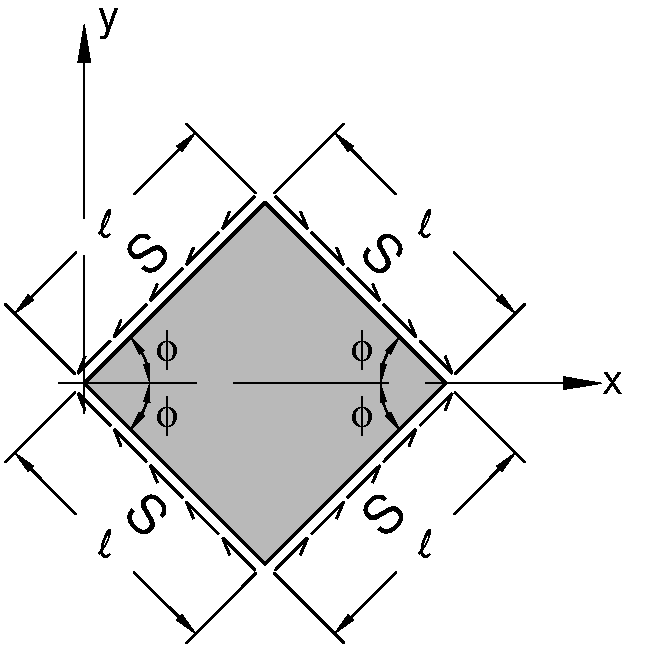
\includegraphics[width=2.8 in]{wedge.pdf}
	\caption{Cuna auto-soportada.}
	\label{wedgee}
\end{figure}


Usando argumentos de equilibrio determinamos que el campo de tensiones solución del problema estaba dado por:

\begin{equation} \label{tencuna}
\begin{split}
& {\sigma _{xx}} = S \cdot Cot\phi \\
& {\sigma _{yy}} =  - S \cdot Tan\phi \\
& {\tau _{xy}} = 0
\end{split}
\end{equation}

Usando las relaciones tensión-deformación para tensión plana (o deformación plana con modulos efectivos) se tiene que:


\[{\varepsilon _{xx}} = \frac{1}{E}\left[ {S \cdot Cot\phi  + \nu  \cdot S \cdot Tan\phi } \right]\]

\[{\varepsilon _{yy}} =  - \frac{1}{E}\left[ {S \cdot Tan\phi  + \nu  \cdot S \cdot Cot\phi } \right]\]

Recordando las relaciones:

\[\left\{ {d\vec u} \right\} = \left[ \varepsilon  \right] \cdot \left\{ {d\vec x} \right\} + \left[ \omega  \right] \cdot \left\{ {d\vec x} \right\}\]

las cuales para el caso plano se simplifican a:

\[du = {\varepsilon _{xx}}dx + \frac{{{\gamma _{xy}}}}{2}dy - \frac{{{\omega _{xy}}}}{2}dy\]

\[dv = {\varepsilon _{yy}}dy + \frac{{{\gamma _{xy}}}}{2}dx + \frac{{{\omega _{xy}}}}{2}dx\]


y reconociendo que por la simetría del problema las componentes rotacionales son nulas se tiene que:

\[u = \int {\frac{1}{E}\left[ {S \cdot Cot\phi  + \nu  \cdot S \cdot Tan\phi } \right]dx}  \equiv \frac{1}{E}\left[ {S \cdot Cot\phi  + \nu  \cdot S \cdot Tan\phi } \right]x + A\]

y

\[v =  - \int {\frac{1}{E}\left[ {S \cdot Tan\phi  + \nu  \cdot Cot\phi } \right]dy}  \equiv  - \frac{1}{E}\left[ {S \cdot Tan\phi  + \nu  \cdot S \cdot Cot\phi } \right]y + B\]

donde $A$ y $B$ son constantes de integración.


\subsection*{Ejemplo 2: Barra sometida a carga axial}

\begin{enumerate}
\item En la \cref{compresion} se muestra una barra de sección rectangular con $a= 40 \;cm$, $b = 50 \;cm$ y longitud inicial $L_{c} = 500$ $cm$, que es  sometida a un ensayo de compresión confinada (está contenida en un recipiente indeformable), mientras que en la \cref{traccion}  se muestra una barra de sección circular con diámetro $d = 50 \;cm$ y longitud inicial $L_{t} =497 \;cm$ sobre la cual se realiza  un ensayo de tracción simple. Las constantes del material, tanto para la barra rectangular como para la barra circular, son $E=150000 \; kgf/cm^2$ y $\nu=0.20$.

Ambos ensayos se realizan con su extremo fijo  en el plano $z = 0$ y están cargados con un sistema que no transmite esfuerzos cortantes y que hace que el esfuezo axial se distribuya uniformemente sobre la superficie transversal de las barras. Los esfuerzos que se inducen a las barras varían con el tiempo conforme a lo mostrado en la figura \cref{carga}
%
\begin{figure}[H]
	\centering
	\subfloat[Barra compresión]{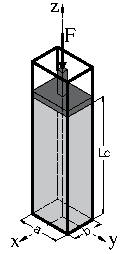
\includegraphics[width=4.0cm]{Compresion.pdf}\label{compresion}}
	\hspace{1 cm}
	\subfloat[Barra tracción]{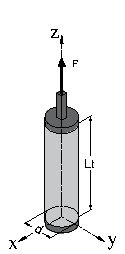
\includegraphics[width=4.0cm]{Traccion.pdf}\label{traccion}}
	\hspace{1 cm}
	\subfloat[Curvas de esfuerzo]{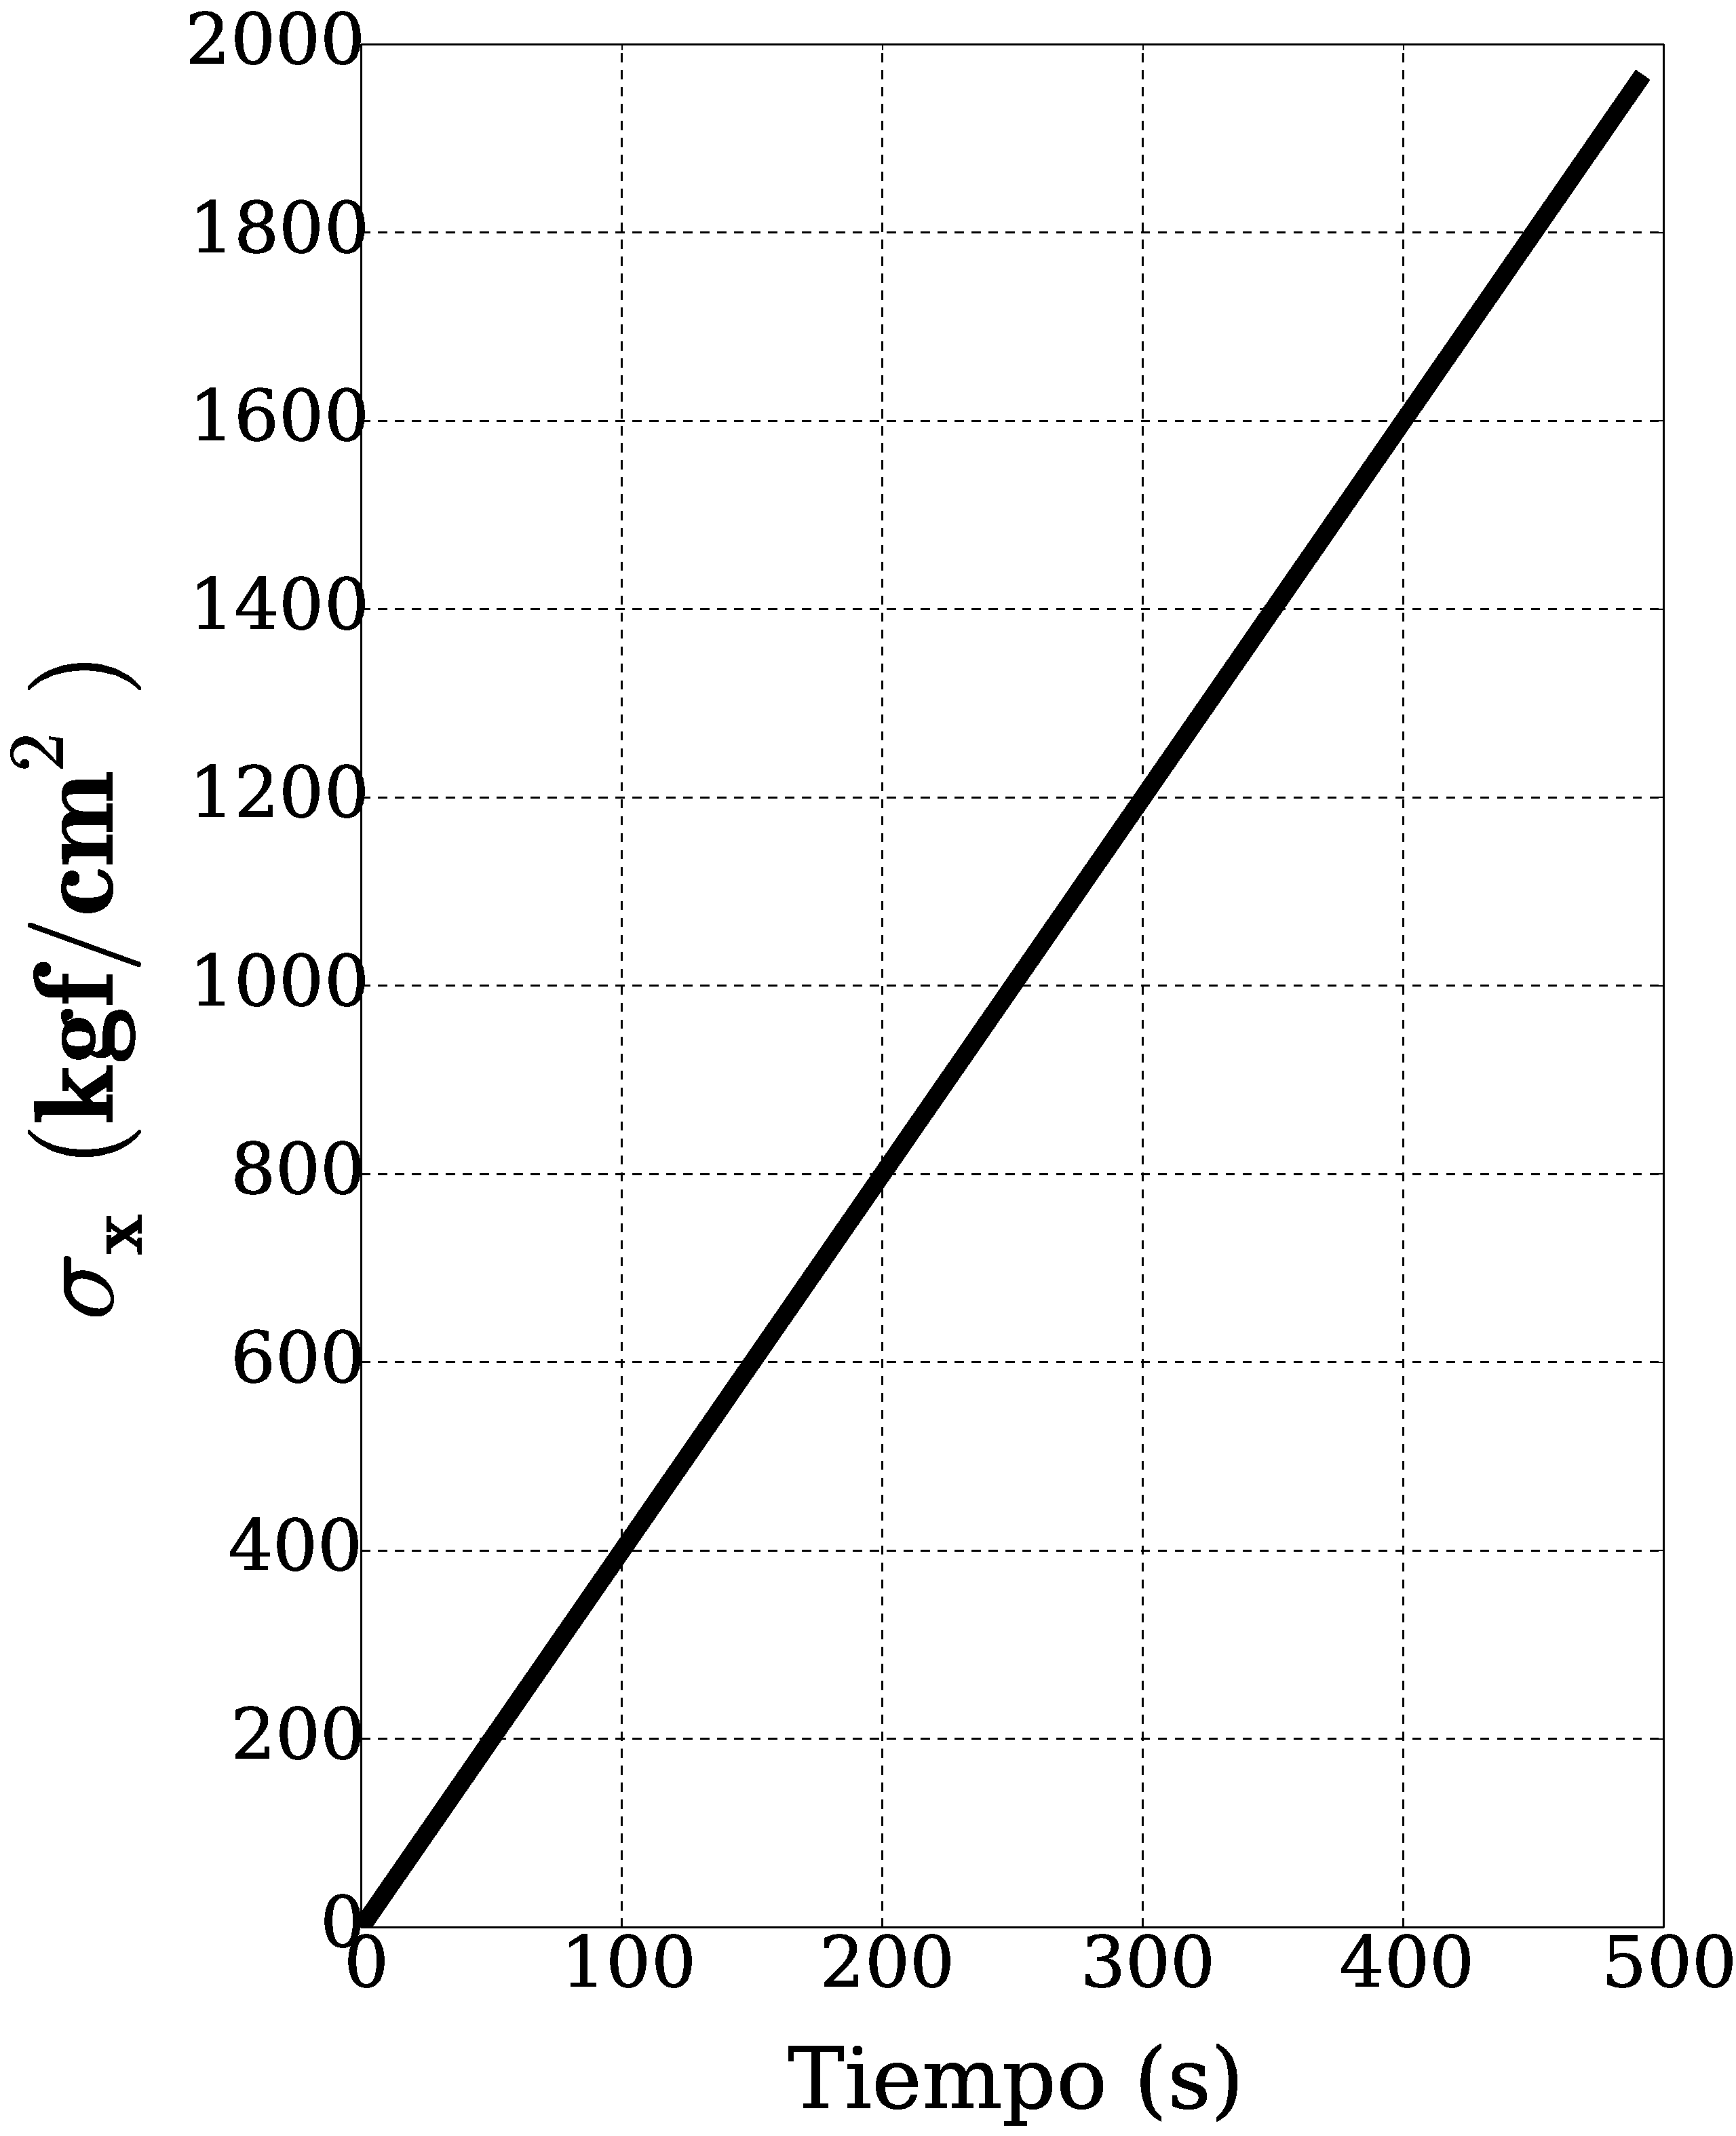
\includegraphics[width=5.5cm]{CurvaEsf.pdf}\label{carga}}
	\caption{Esquema ensayos y curvas de apliación carga}
	\label{ensayo}
\end{figure}

Determine: 
\begin{itemize}
	\item ¿Cuál es el tiempo $t$ en el cual las dos barras tienen la misma longitud? \\
	
	\textbf{Solución:}\\
	
	La barra circular está solamente sometida a esfuerzo axial $\sigma_{zz}$, por lo que la deformación es: 
	
	\[\varepsilon _{zz_t} = \dfrac{\sigma_{zz_t} }{E}\] 
	
	y la longitud final sería: 
	
	\begin{equation}
	\begin{split}
	{L_{f_{cir}}} & = L_{ini_{cir}} (1+  \varepsilon _{zz_t} ) \\\\
	{L_{f_{cir}}} & = L_{ini_{cir}} \left(1+  \dfrac{\sigma_{zz_t} }{E}\right) \\
	\end{split}
	\label{trac}
	\end{equation}
	
	Por otro lado, la barra cuadrada está sometida a esfuerzo axial $\sigma_{xx}$, $\sigma_{yy}$ y $\sigma_{zz}$, pero solo se deforma en el eje $z$ que es la deformación de interés. Para este caso entonces: \\
	
	\[\varepsilon _{zz_c} = \dfrac{\sigma_{zz_c} }{(2 \mu + \lambda)}\] \\

donde $\mu =   \left(\dfrac{E }{2(1 + \nu)}\right)$  y $\lambda =   \left(\dfrac{\nu{E} }{(1 + \nu) (1 - 2\nu)}\right)$. \\

	llamando $A = (2 \mu + \lambda)$ se tiene que la longitud final para la barra cuadrada sería: 
	
	\begin{equation}
	\begin{split}
	{L_{f_{cua}}} & = L_{ini_{cua}} (1+  \varepsilon _{zz_c} ) \\\\
	{L_{f_{cua}}} & = L_{ini_{cua}} \left(1+  \dfrac{\sigma_{zz_c} }{A}\right) \\
	\end{split}
	\label{comp}
	\end{equation}
	
Lo que queda sería entonces igualar las longitudes y despejar el tiempo. Para hacer esto, es preciso tener en cuenta barra circular es cargada solo hasta que el esfuerzo es $\sigma=350  \; kgf/cm^2$ por lo que habrá que considerar ambas condiciones. Por simplicidad inicialmente determinemos que pasaría si $t > 350 s$, es decir en donde $\sigma_{zz_t} = 350  \; kgf/cm^2$. Reemplazando el valor de los esfuerzos en función del tiempo en la \cref {trac} y la  \cref{comp}

	\begin{equation}
	\begin{split}
	{L_{f_{cir}}} & = 497 \left(1+  \dfrac{350 }{E}\right) \\
	\end{split}
	\label{trac2}
	\end{equation}	
		\begin{equation}
	\begin{split}
	{L_{f_{cua}}} & = 500 \left(1- \dfrac{t }{A}\right) \\
	\end{split}
	\label{comp2}
	\end{equation}

donde $A \simeq 1.1111E$ \\

	Igualando la \cref {trac2} y la  \cref{comp2} y despejando $t$ se obtiene: 
	
	\[t=613.4 \; s\]
	
	
	\item En la barra circular, ¿cuáles son los desplazamientos y las deformaciones en el punto de coordenadas $(x,y,z) = (20,15,450) \; cm$ para el tiempo $t = 300 \;s$?  \\

Las deformaciones asociadas a la barra son:  
%
	\begin{equation}
	\begin{split}	
	{\varepsilon _{xx_t}} &= -\nu \dfrac{\sigma_{zz_t} }{E} \\\
	{\varepsilon _{yy_t}} &= -\nu \dfrac{\sigma_{zz_t} }{E} \\\
	{\varepsilon _{zz_t}} &= \dfrac{\sigma_{zz_t} }{E} 
	\end{split}
	\label{defpto2}
	\end{equation}
%	
reemplazando $\sigma_{zz_t}$ por 300
%
	\begin{equation}
	\begin{split}
	{\varepsilon _{xx_t}} &= -0.0004 \\
	{\varepsilon _{yy_t}} &= -0.0004 \\
	{\varepsilon _{zz_t}} &= 0.002
	\end{split}
	\label{defpto2sol}
	\end{equation}

Por otro lado para determinar los desplazamientos integramos la deformación. Por ser deformación constante la integración se obtiene multiplicando la deformación por las distancias hasta el punto de evaluación. 
%
	\begin{equation}
	\begin{split}
	{u} &= -0.0004 (20  \;cm) = -0.008 \;cm \\
	{v} &= -0.0004 (15  \;cm) = -0.006 \;cm  \\
	{w} &= 0.002  (450  \;cm) = 0.9  \; cm 
	\end{split}
	\label{defpto2sol}
	\end{equation}

	\item   ¿Cuál es el valor del máximo esfuerzo cortante en un punto al interior de la barra rectagular durante el ensayo? \\

Los esfuerzos para la barra cuadrada están dados por 
%
	\begin{equation}
	\begin{split}	
	{\sigma_{xx_c}} &=   \lambda \varepsilon _{zz_c} \\
	{\sigma_{yy_c}} &=   \lambda \varepsilon _{zz_c} \\
	{\sigma_{zz_c}} &=  (2\mu + \lambda) \varepsilon _{zz_c}
	\end{split}
	\label{defpto2}
	\end{equation}

El corte máximo se da entonces: 

\[\tau_{max} = \varepsilon _{zz_c}  \left(\dfrac{2\mu + \lambda - \lambda}{2}\right)\]

llamando de nuevo $A = (2 \mu + \lambda)$

\[\tau_{max} = \sigma_{zz_c} \left(\dfrac{\mu}{A}\right)\]

para  $\sigma_{zz_c} = 1000 \; kgf/cm^2$

\[\tau_{max} = 1000 \left(\dfrac{\mu}{A}\right) \; kgf/cm^2\] 

\end{itemize}

\end{enumerate}

\section{Ejercicios}


\begin{enumerate}

\item \label{punto01_m} Para un campo de desplazamientos dado por:
\[\mathbf{u} = a(x^2 - 5y^2)\hat{\mathbf{i}} + (2ax y)\hat{\mathbf{j}} \]

\begin{enumerate}
\item Determinar el tensor de deformaci\'on
\item Obtener las deformaciones principales
\item Obtener los esfuerzos principales
\end{enumerate}

\item \label{punto02_m}  En la  \cref{columna_CargaP} se muestra una columna prism\'atica, de secci\'on cuadrada (lado $a$), con una tracci\'on axial igual a $P$. Si el material del que est\'a hecha la pieza tiene propiedades $\nu$ y $E$, encontrar los campos de esfuerzos y deformaciones.
\begin{figure}[H]
	\centering
	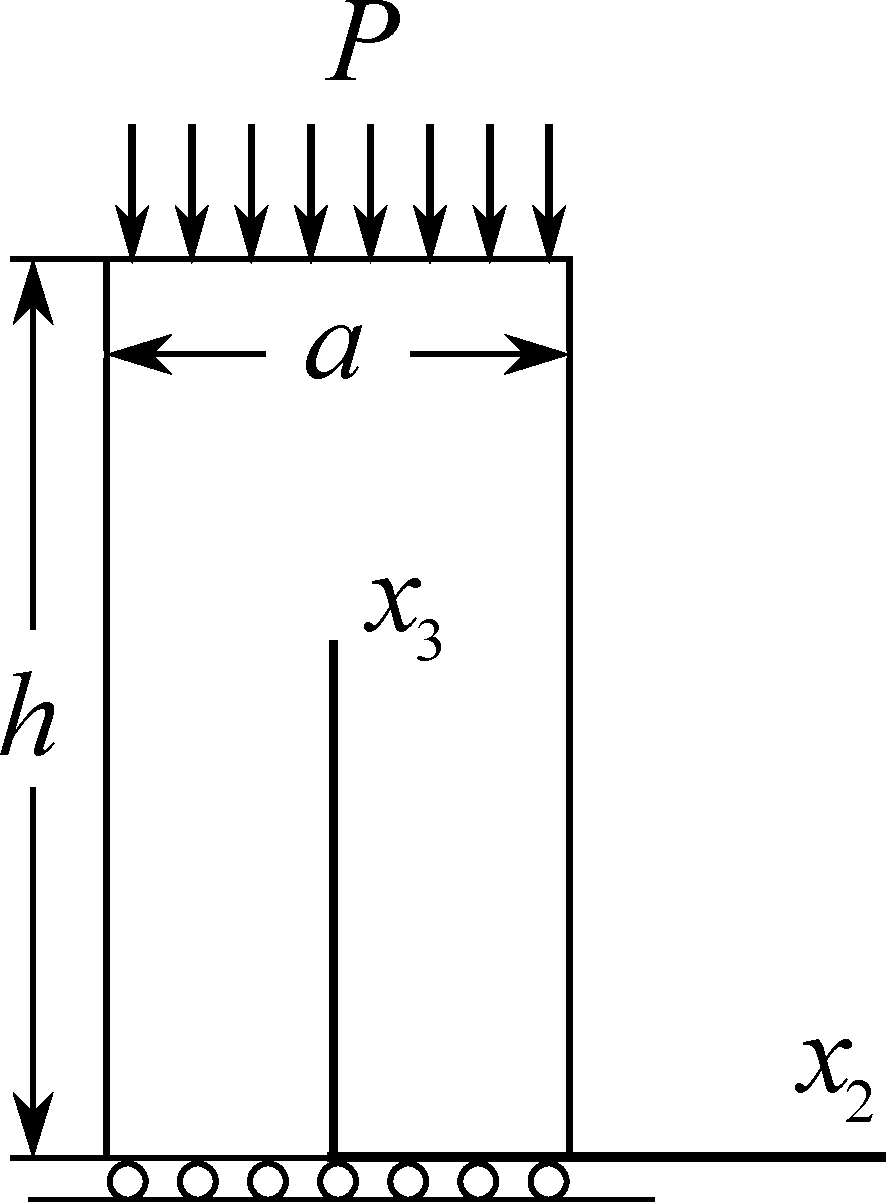
\includegraphics[height=5cm]{columna_CargaP.pdf} 
	\caption{Columna con carga axial.}
	\label{columna_CargaP}
\end{figure}

\item \label{punto03_m} En la \cref{fig:columna_g} se muestra la misma columna  del ejercicio anterior, pero en este caso se quiere estudiar la deformaci\'on causado por su propio peso. Si las componentes del tensor de esfuerzos son:
\begin{align*}
&\sigma_{33} = \rho g(h- x_{3}) \enspace ,\\
&\sigma_{11} = \sigma_{22} = 0 \enspace ,\\
&\sigma_{12} = \sigma_{13} = \sigma_{23} = 0 \enspace .
\end{align*}

\begin{figure}[h]
	\centering
	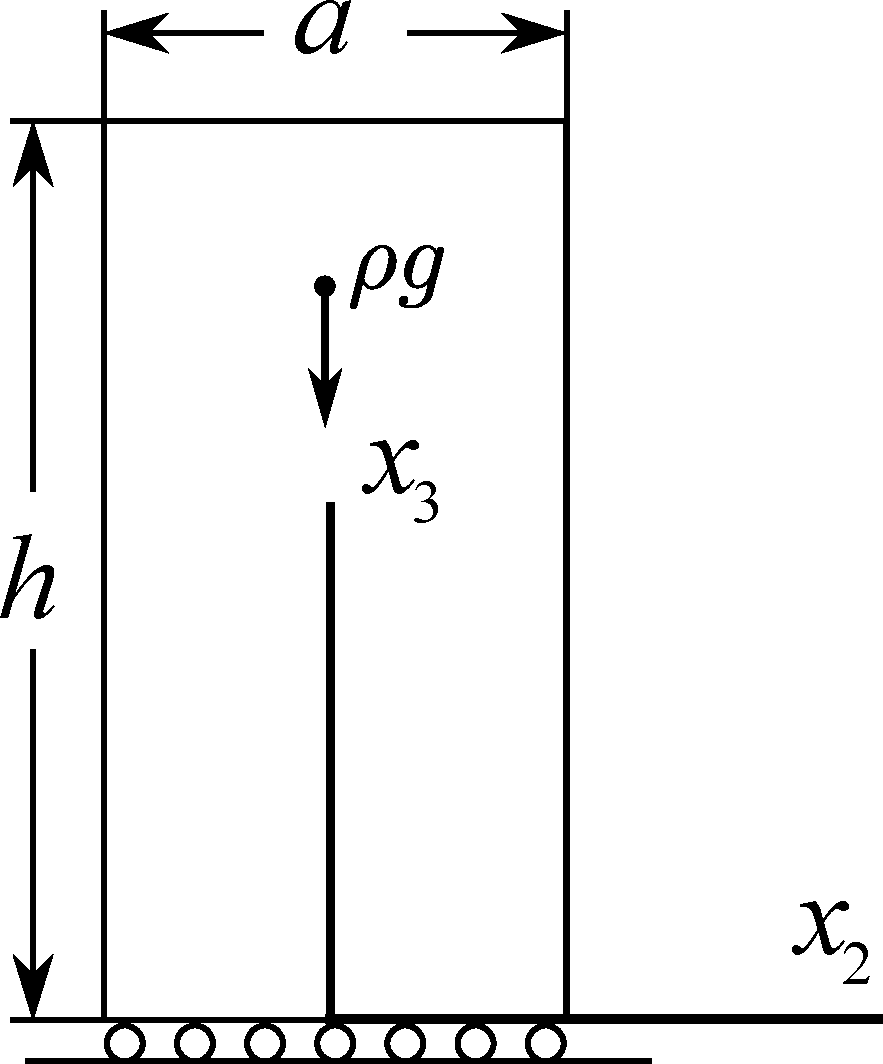
\includegraphics[height=4.5cm]{columna_Peso.pdf} 
	\caption{Columna bajo la acci\'on de su propio peso.}
	\label{fig:columna_g}
\end{figure}

\begin{enumerate}
\item Calcular los campos de deformaciones si las propiedades del material son $\nu$ y $E$.
\end{enumerate}
\newpage
\item \label{punto04_m}En la  \cref{fig:viga} se muestra una viga en voladizo de secci\'on unitaria con una carga distribuida en su extremo de forma parab\'olica.
\[\mathbf{t} = \frac{Pc^2}{2I}\left(1-\frac{y^2}{c^2}\right)\hat{\mathbf{j}}\].La soluci\'on para esfuerzos es de la forma
\begin{align*}
&\sigma_{xx} = -\frac{P}{I}xy \enspace ,\\
&\sigma_{yy} = 0 \enspace ,\\
&\sigma_{xy} = -\frac{P}{2I}(c^2 - y^2) \enspace .
\end{align*} \\

Y para el campo de desplazamientos es:
\begin{align*}
&u_{x} = \left(\frac{1}{G} - \frac{\nu}{E}\right)\frac{Py^3}{6I} + \left(\frac{l^2}{E} - \frac{x^2}{E} - \frac{c^2}{G} \right)\frac{Py}{2I} \enspace ,\\
&u_{y} = \frac{\nu P xy^2}{2EI} + \frac{Px^3}{6EI} - \frac{Pl^2x}{2EI} + \frac{Pl^3}{3EI} \enspace ,
\end{align*} \\
en donde $G=E/(2 + 2\nu)$ es el m\'odulo de cortante e $I$ es el momento de inercia.

\begin{figure}[h]
	\centering
	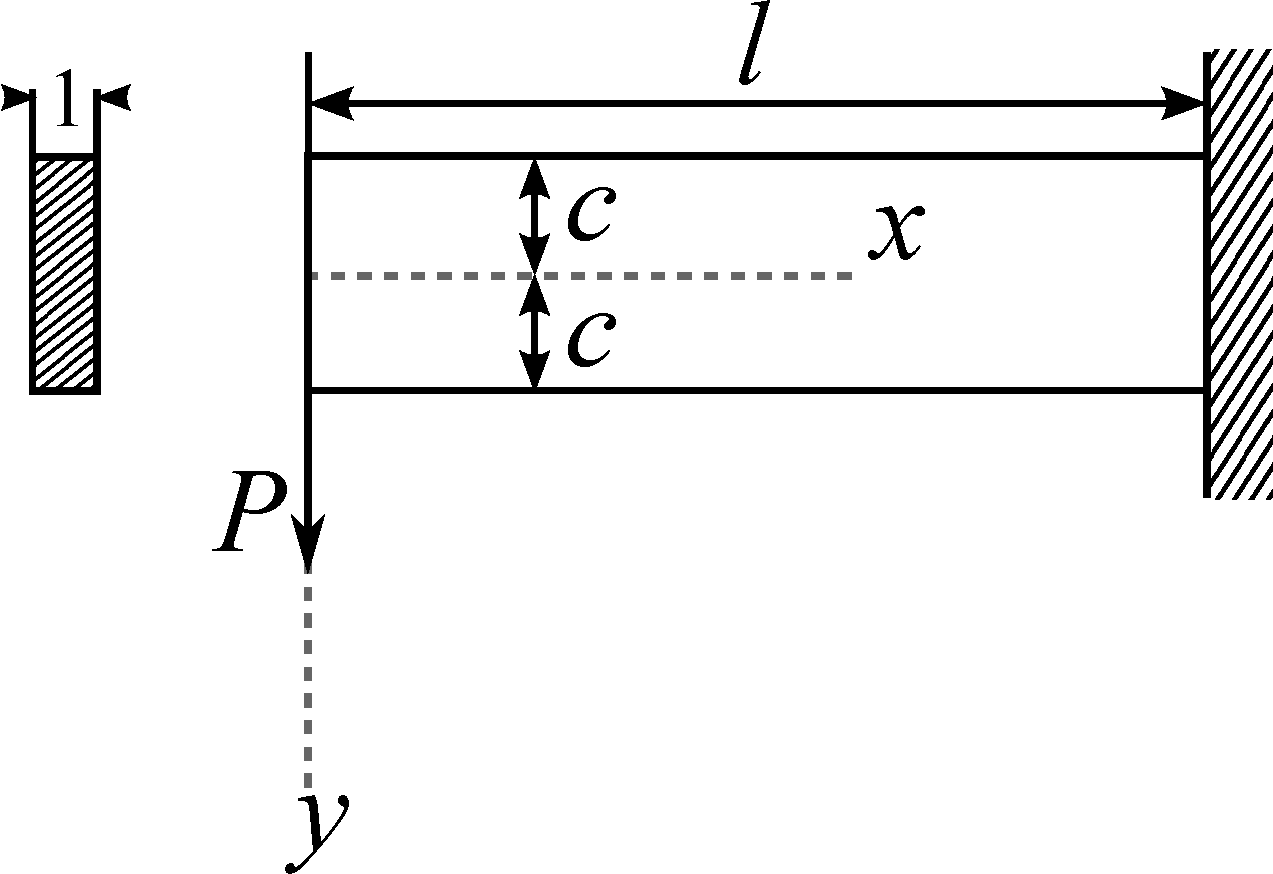
\includegraphics[height=5cm]{Viga_Voladizo.pdf} 
	\caption{Viga en voladizo con una carga distribuida en su extremo.}
	\label{fig:viga}
\end{figure}

\begin{enumerate}
\item Determinar las condiciones de frontera del problema.
\item Verificar que las soluciones de esfuerzos y desplazamientos satisfacen las condiciones de frontera.
\item Encontrar la regi\'on de la viga que est\'a a compresi\'on y la regi\'on tensi\'on, y por tanto el eje neutro. Y determinar la ecuaci\'on de desplazamientos para este eje neutro. Comparar con la teor\'ia cl\'asica de vigas.
\end{enumerate}

\newpage
\item \label{punto05_m} En la  \cref{bloques} se muestra un paralelep\'ipedo de dimensiones $a$, $b$ , $c$, constituido por un material homog\'eneo el\'astico y lineal se aloja en una cavidad de la misma forma y dimensiones, cuyas paredes son de un material lo suficientemente r\'igido para poderlo suponer indeformable.
Sobre la abertura de la cavidad de dimensiones $a\times b$ y a trav\'es de una placa r\'igida de peso y rozamiento despreciables se aplica, perpendicularmente a ella, una fuerza $F$ que comprime al bloque el\'astico. \footnote{Tomado del ejemplo 3.5 en Chávez, E. Problemas resueltos de mecánica del medio Continuo}

Calcular:
\begin{enumerate}
\item Las fuerzas laterales ejercidas por las paredes de la cavidad sobre el paralelep\'ipedo;
\item La variaci\'on de altura experimentada por el mismo.
\end{enumerate}

\begin{figure}[h]
	\centering
	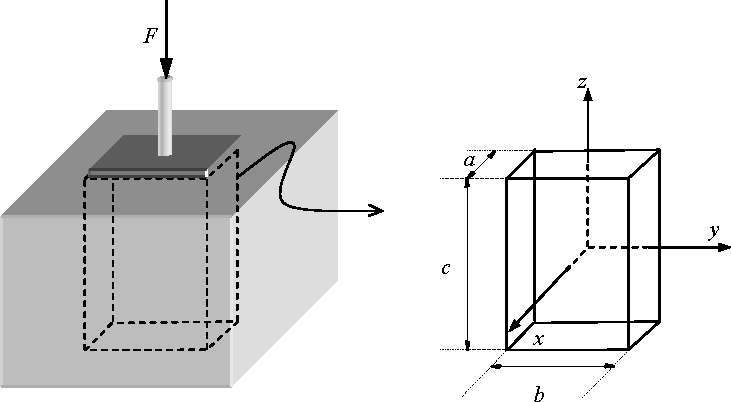
\includegraphics[height=8cm]{bloques.pdf} 
	\caption{Paralelepípedo}
	\label{bloques}
\end{figure}

\item \label{punto06_m} En un punto de un suelo que podemos considerar como un s\'olido el\'astico lineal se conoce la deformaci\'on volum\'etrica $\epsilon_V = -2\times10^{-3}$ , la deformaci\'on tangencial $\epsilon_{xy} = - 3 \times 10^{-3}$ y la deformaci\'on  $\epsilon_{xx} = 0$ . El suelo est\'a sometido a un estado de deformaci\'on plana en el plano $x y$. Se pide:
\begin{enumerate}
\item Componentes cartesianas del tensor de deformaci\'on. 
\item  Suponiendo que las constante el\'asticas son $E = 50$MPa , $\nu =1/4$ , obtener las componentes del tensor de tensiones y sus valores principales. Obtener asimismo las direcciones en las que las tensiones normales y tangenciales son m\'aximas o m\'inimas y sus valores.
\end{enumerate}

\item \label{punto07_m} Un s\'olido se halla sometido a deformaci\'on plana, siendo las componentes del tensor de deformaci\'on en un punto: 
\[\overset{\rightarrow (2)}\epsilon = \left[ \begin{array}{ccc}
-2 & 3 & 0 \\ 
3 & -10 & 0 \\ 
0 & 0 & 0
\end{array}  \right] \times 10^{-3}\]
Considere que el s\'olido tiene un comportamiento el\'astico lineal e is\'otropo, definido por
m\'odulo el\'astico de Young $E = 10$MPa y coeficiente de Poisson $\nu = 0.25$ .
Se pide:
\begin{enumerate}
\item Obtener las deformaciones principales y las direcciones en que se producen;
\item Obtener las componentes del tensor de tensiones de Cauchy;
\item Obtener las m\'aximas y m\'inimas tensiones normales;
\item Se sabe que el material rompe cuando en alg\'un plano se alcanza una tensi\'on tangencial
que supere $40$ kPa. Verificar si se produce la rotura.
\end{enumerate}

\item \label{punto08_m}  En la \cref{barcomp}  se muestra una barra, de sección rectangular, $a= 40$ $cm$, $b = 50$ $cm$ y longitud inicial $L_{c} = 500$ $cm$, que es  sometida a un ensayo de compresión confinada (está contenida en un recipiente indeformable). En la \cref{bartrac} se muestra una barra, de sección circular, de diámetro $d = 50$ $cm$ y longitud inicial $L_{t} =497$ $cm$ sobre la cual se realiza  un ensayo de tracción simple. Las constantes del material, tanto para la barra rectangular como para la barra circular, son $E=150000$ $kgf/cm^2$ y $\nu=0.20$.

Ambos ensayos se realizan con su extremo fijo  en el plano $z = 0$ y están cargados con un sistema que no transmite esfuerzos cortantes y que hace que el esfuezo axial se distribuya uniformemente sobre la superficie transversal de las barras. Los esfuerzos que se inducen a las barras varían con el tiempo, conforme a lo mostrado en la  \cref{time}
%
\begin{figure}[H]
	\centering
	\subfloat[Barra compresión]{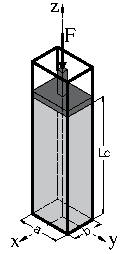
\includegraphics[width=4.0cm]{Compresion.pdf} \label{barcomp}}
	\hspace{0.5 cm}
	\subfloat[Barra tracción]{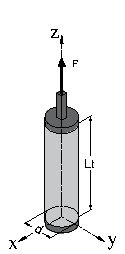
\includegraphics[width=4.0cm]{Traccion.pdf}\label{bartrac}}	
	\hspace{0.5 cm}
	\subfloat[Curvas de esfuerzo]{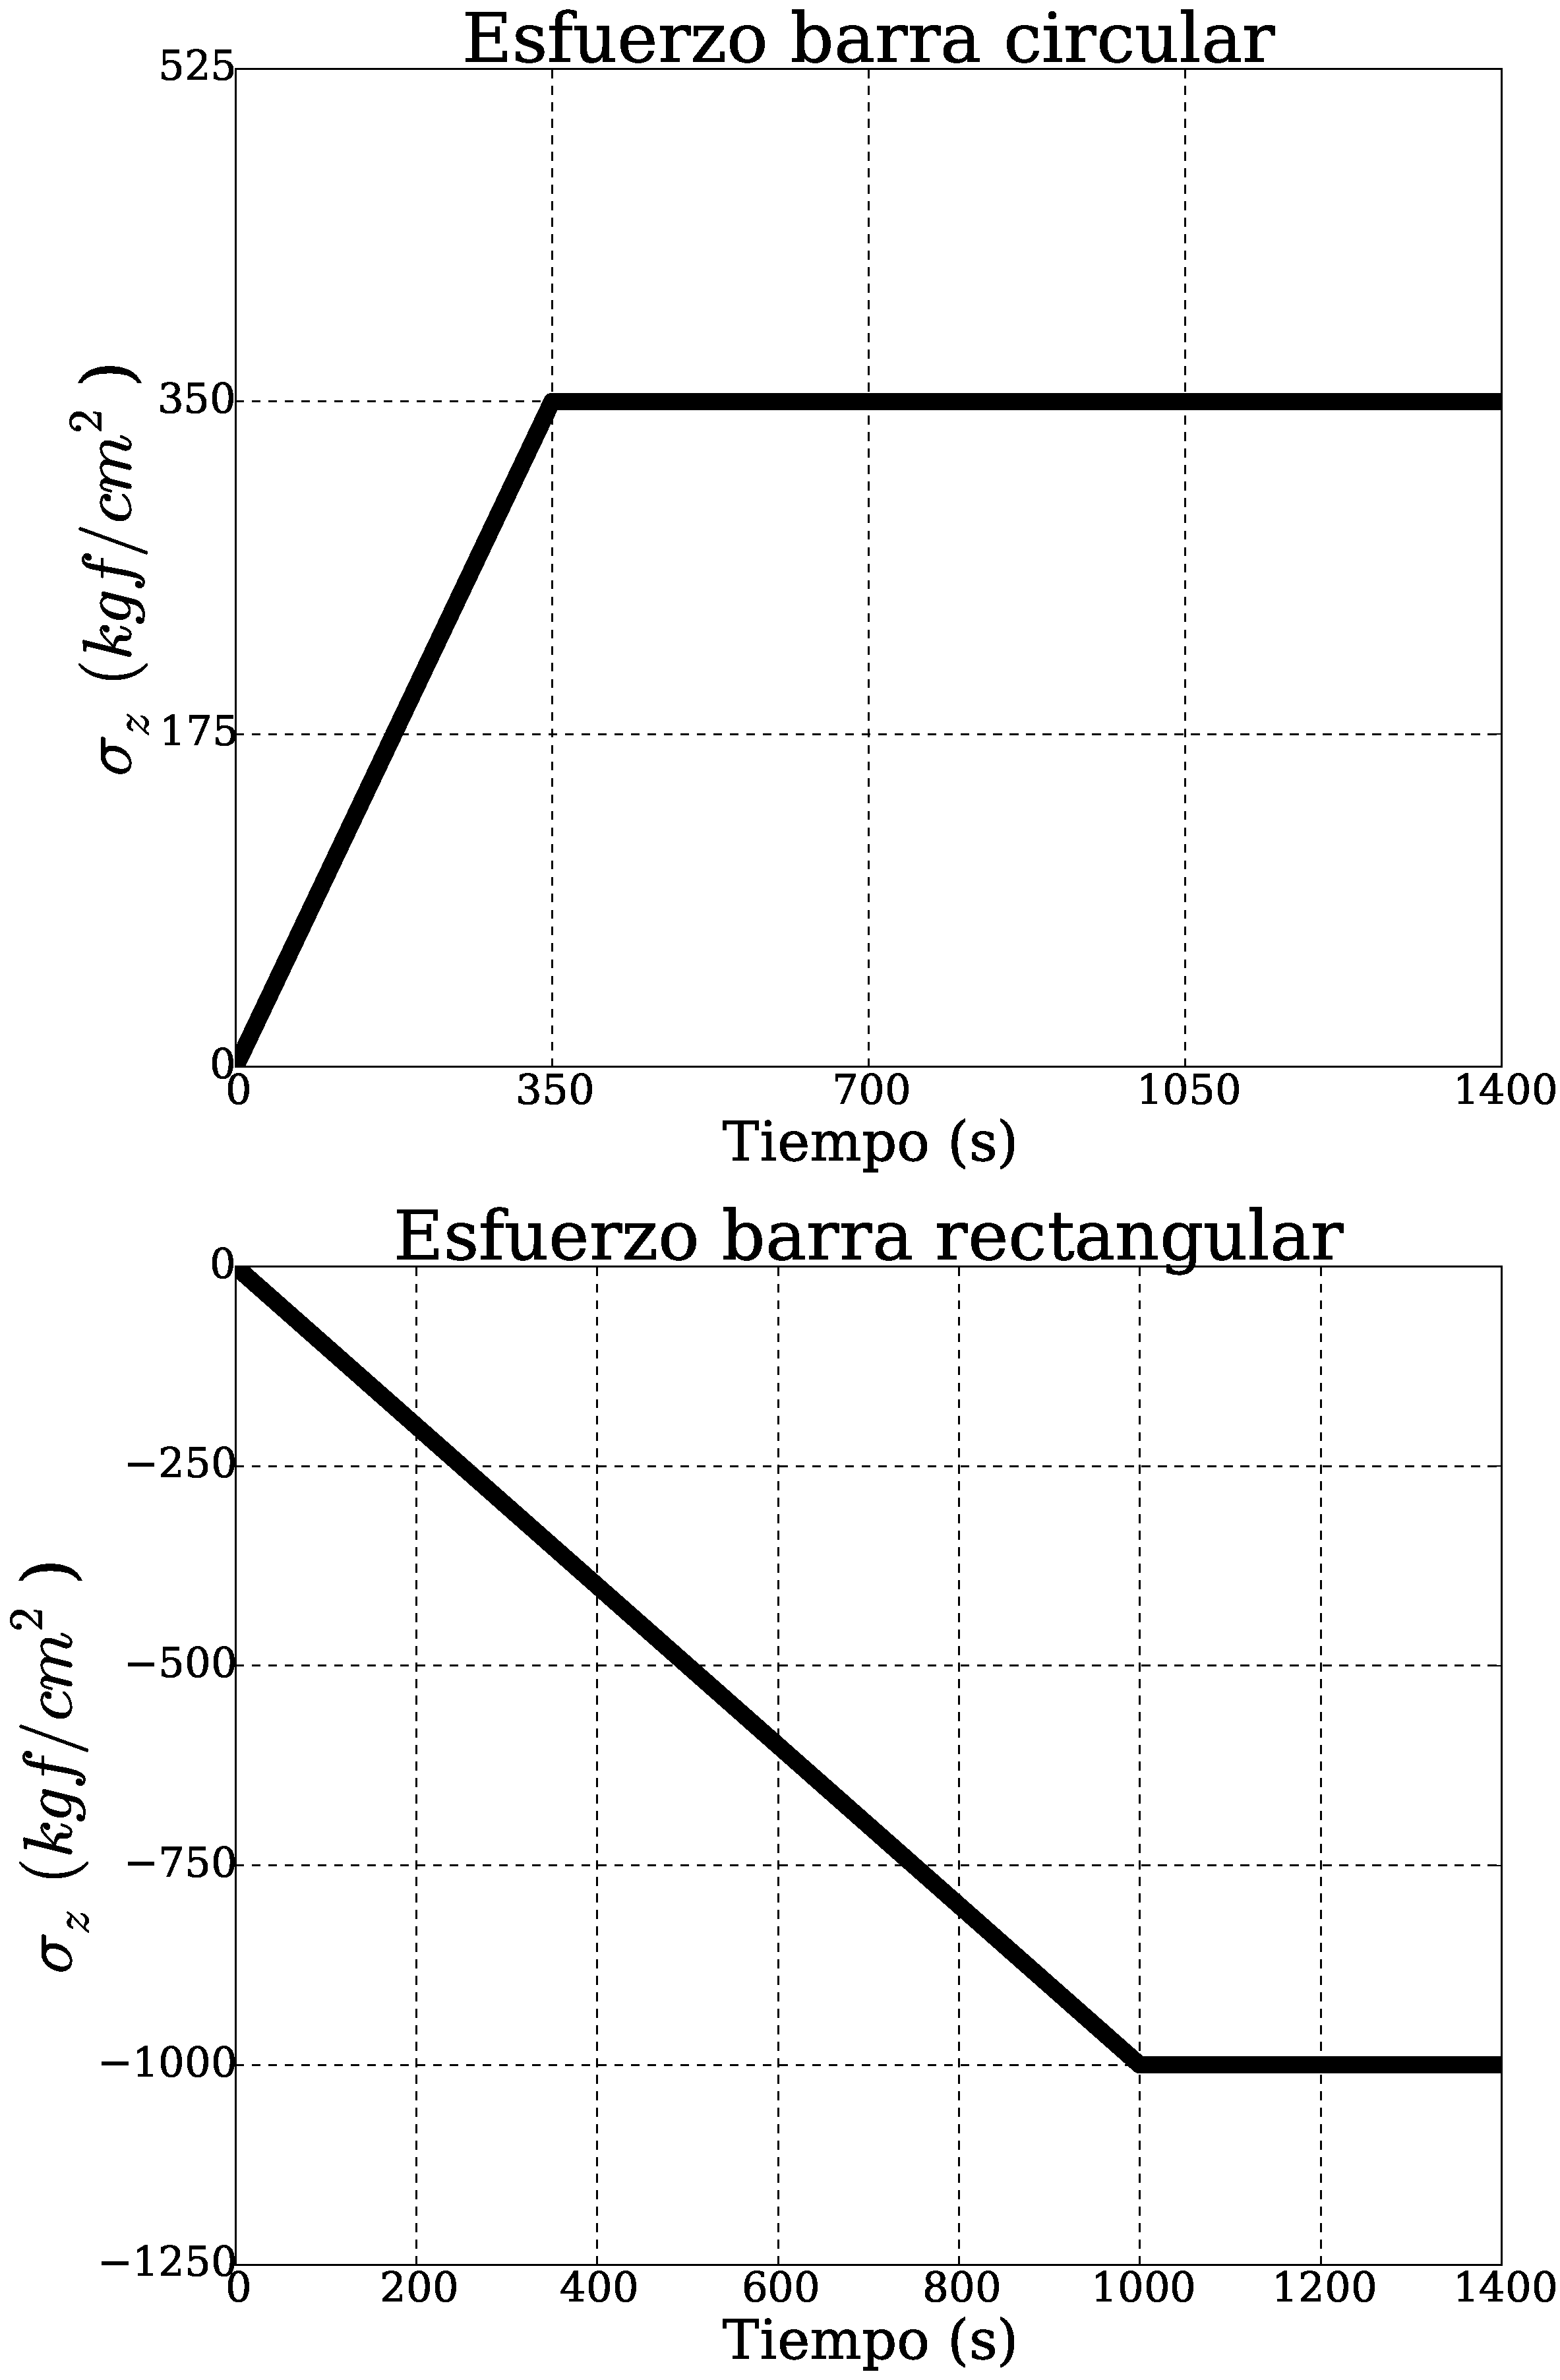
\includegraphics[width=6.0cm]{Esftime.pdf}\label{time}}
	
	\caption{Esquema ensayos y curvas de apliación carga}
	\label{ensayo}
\end{figure}

\begin{enumerate}
	\item ¿Cuál es el tiempo $t$ en el cual las dos barras tienen la misma longitud? \\	
	\item En la barra circular, ¿cuáles son los desplazamientos $u$, $v$ y $w$ y las deformaciones $\varepsilon_{xx}$ $\varepsilon_{yy}$ y $\varepsilon_{zz}$ en el punto de coordenadas $(x,y,z) = (20,15,450)$ $cm$ para el tiempo $t = 300$ $s$? 
	\item ¿Cuál es el valor del máximo esfuerzo cortante en un punto al interior de la barra rectagular durante el ensayo? 	
	\item  ¿Cuál es el área mínima que alcanza la sección transversal de la barra circular durante el ensayo?
	\item  ¿En la barra rectuangular, en el tiempo $t=1000$ $s$ cuál son las fuerzas $F_x$ y $F_y$ que le transmite la barra a las paredes del recipiente?
\end{enumerate}

\newpage
\item En la \cref{placa} se presenta una placa en forma de rombo sometida a la acci\'on de una carga, en el plano $XY$, que se encuentra distribuida sobre su per\'imetro y cuyo campo de desplazamientos está dado por:

$A$ es una constante positiva, $E$  es el módulo de elasticidad del material y $\nu$ la relación de Poisson.

$ u \left(x,y,z \right) =  \dfrac{A}{E}  \left(1 - \nu \right) x$ \hspace*{5mm}
$ v \left(x,y,z \right) = \dfrac{A}{E}  \left(1 - \nu \right) y$	\hspace*{5mm} 
$ w \left(z \right) = -\dfrac{2A \nu}{E} z$ \\\\
%
\begin{figure}[H]
	\centering
	\subfloat[Placa]{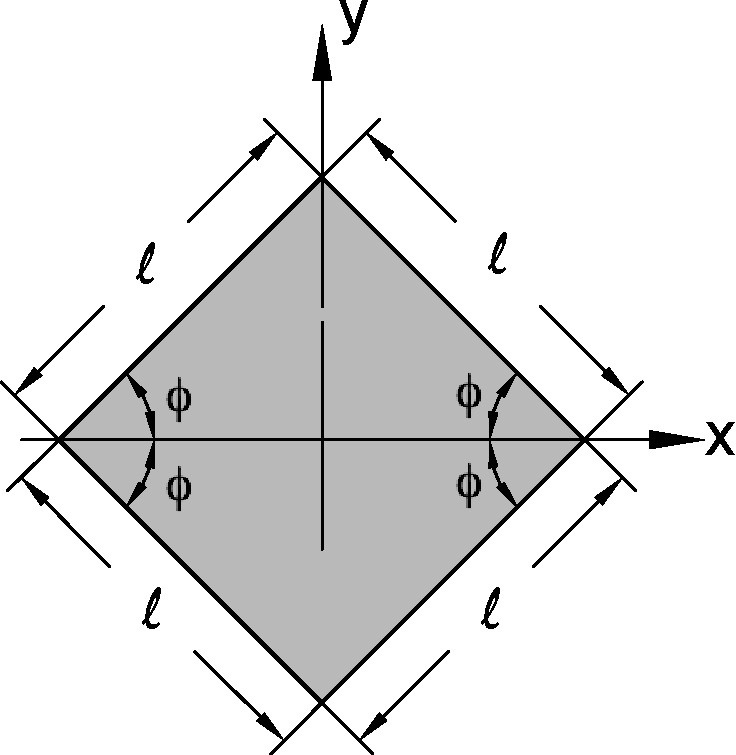
\includegraphics[width=2.5in]{cuna.pdf}\label{placa}}
	\hspace{2 cm}
	\subfloat[Esquema para dibujar las cargas axiales y tangenciales]{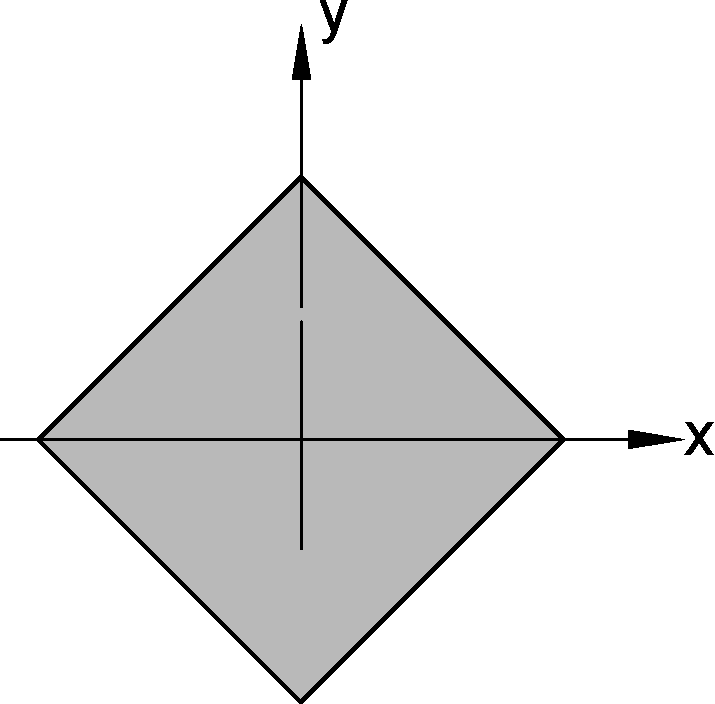
\includegraphics[width=2.5in]{cunanada.pdf}\label{esquema}}
	%\label{placa}
\end{figure}
%
\begin{itemize}
	%
	\item Determine la deformaci\'on unitaria axial m\'axima $\varepsilon$ y la deformac\'on angular m\'axima {\Large{$\gamma$}} que se presentan en la placa.¿En qu\'e puntos se presentan?.
	\item Dibujar la configuraci\'on deformada de la placa en el plano $xy$. ¿Cu\'ales son los puntos que experimentan los m\'inimos desplazamientos?.
	\item Ilustre la deformaci\'on de la part\'icula con coordenadas $\left( \dfrac{l}{4}, 0, 0 \right)$ en el plano $xy$. Utilice cuadrados de tama\~no diferencial.
	\item Determine y represente gr\'aficamente, sobre la figura (b), la tensi\'on normal y tangencial a la cara de la placa, contenida en el cuadrante I del plano $XY$.
\end{itemize}



\end{enumerate}

\end{document}
